\section{Pilotforsøg}
I dette bilag beskrives pilotforsøgets fremgangsmåde, samt hvilke resultater der opsamles under udførelsen heraf. 

\subsection{Formål}
Dette pilotforsøg har til formål at kunne præcisere samt optimere kravspecifikationerne i de enkelte blokke, hvorved uklare parametre forventes at kunne besvares. Disse parametre omfatter identificering af støj signaler, EMG-signalets frekvensområde samt elektrodernes placering. Parametrene vil forsøges besvaret udfra målinger ved udførelse af en squat-øvelse.
Hertil anvendes en EMG-forstærker og et accelerometer som sensorer. På baggrund af dette opstilles følgende formål for de enkelte sensorer.  

\subsubsection{EMG-forstærker}
\begin{enumerate}
\item Opsamling af signal fra rectus femoris og biceps femoris
\begin{itemize}
\item Identificering af elektrodernes placering
\item Sammenligning af muskelaktivitet oprejst og i en squat-øvelse 
\end{itemize}
\item Identificering af støjsignaler
\item Identificering af frekvensområde
\item Identificering af gain til mikroprocesserens operationsspænding
\end{enumerate}

\subsubsection{Accelerometer}
\begin{enumerate}
\item Identificering af knæleddets position siddende i en squat-øvelse
\item Identificering af støjsignaler
\end{enumerate}

\subsection{Materialer} 
\begin{itemize}
\item EMG-forstærker
\item Elektroder %Hvilke elektroder?
\item Desinfektionsservietter
\item Skraber
\item Tusch 
\item Accelerometer ADXL335Z
\item Tape
\item Ledninger %Hvilke ledninger?
\item Computer
\item CY8CKIT-042-BLE
\end{itemize}

\subsection{Metode}
For at identificere den bedst mulige elektrodeplacering tages der udgangspunkt i den anatomiske afbildning af låret, som ses af \autoref{fig:laarmuskler}.

\begin{figure}[H]
\centering
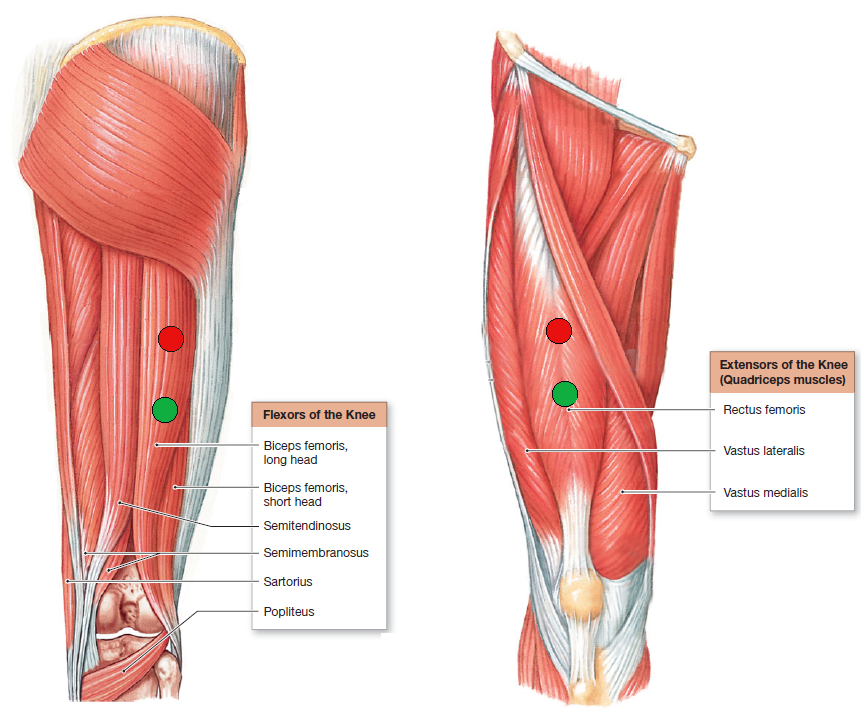
\includegraphics[width=0.5\textwidth]{figures/laarmuskler.png}
\caption{Biceps femoris og rectus femoris \citep{martini2012}.}
\label{fig:laarmuskler}
\end{figure}

Elektroderne placeres medialt for både rectus femoris samt biceps femoris for så vidt muligt, at elektroderne forbliver over musklen ved en kontraktion. 

Da der ikke fremgår nogen muskel på den superiore mediale del af tibia, benyttes dette som referencepunkt for EMG-målingen, hvortil der forventes en stabil reference. 

Til identificering af støj fra EMG-forstærkeren fortages der baselinemålinger, som senere analyseres via en frekvensanalyse. Det samme gør sig gældende for identificeringen af EMG-signalets frekvensområde, dog vil dette være under udførelsen af en squat-øvelse.  

%Evt. noget med gain..

For at simulere den påvirkning som accelerometeret udsættes for og derved identificere det maksimale og minimale outputsignal roteres accelerometeret i en langsom rotation fra 0$^{\circ}$ til 90$^{\circ}$ både til højre og venstre. Herudover måles accelerometerets påvirkning i henholdsvis 0 og 1 g-påvirkning for at identificere accelerometeres påvirkning samt, hvorvidt dette stemmer overens med databladet. 

\subsection{Forsøgsopstilling}
Forsøgsopstilling er for den primære udførelse af forsøget. Nogle af processerne gentages for at kunne sammenligne de forskellige målinger, og derved få et bedre resultat.
% Omskriv..

\subsubsection{EMG-forstæker}
Rectus femoris og biceps femoris identificeres, den ønskede placering af elektroderne markeres med tusch. Der fjernes eventuelle hår og døde hudceller ved brug af skraber. Huden desinficeres herefter ved brug af desinficeringsservietter og elektroderne påsættes. 
Til forsøget benyttes to EMG-forstærkere og dermed to elektrode sæt, bestående af en positiv-, negativ- samt en referenceelektrode. Det ene sæt påsættes rectus femoris og det andet på biceps femoris. Referenceelektroderne fra sættene placeres superiort medialt på tibia. 

\subsubsection{Accelerometer}
Accelerometeret placeres lateralt på låret, således accelerometeret måles i xyz-plan, hvorved der måles i den vertikale retning. Der sørges for, at accelerometeret befinder sig i 0 g-påvirkning ved starten af forsøgets udførelse, hvorved accelerometeret er kaliberet. 
% Det at der måles vertikalt i xyz-planet fatter vi ikke!

\subsubsection{Opstilling}
\begin{itemize}
\item Identificering af musklerne rectus femoris og biceps femoris 
%\item Elektrodernes placering markeres
\item Huden prepereres
\item Elektroderne påsættes
\item Ledningerne påsættes elektroderne
	\begin{itemize}
	\item Elektrodesæt 1: positiv og negativ på rectus femoris
	\item Elektrodesæt 2: positiv og negativ på biceps femoris
	\item Fælles reference på tibia
	\end{itemize} 
\item Accelerometeret påsættes patella ved en 0 g-påvirkning i xyz-retning
% Hvor placeres accelerometeret??? Et sted står der lateralt på låret (afsnittes før, linje 70) og linje 85/herover, står noget andet.
\end{itemize}


\subsection{Fremgangsmåde}
Fremgangsmåden udføres XX antal gange, hvorved der på baggrund af målingerne foretages en gennemsnitsværdiberegning.
%Bruges til hvad? Er dette med henblik på at lave en standardafvigelse senere, eller???

\subsubsection{EMG-forstærker}
EMG-måling: 10-sekunders målinger trinvist under udførelse af en squat-øvelse. 


\subsubsection{Accelerometer}
Påvirkning i henholdsvis 0$^{\circ}$ og 90$^{\circ}$.
Påvirkning af rotation fra $0-90^{\circ}$ både til højre og venstre.
Samplingstid 30 sekunder ved henholdsvis 0$^{\circ}$ og 90$^{\circ}$ .
Optag rotation: baseline 10 sekunder, rotation 10 sekunder, baseline 10 sekunder % Hvad er det for en rotation??/Hvordan rotation??? 


